\documentclass[../DatenbankenFS23.tex]{subfiles}

\begin{document}
\section{Die Mengenlehre}
\subsection{Objekte in der Mengenlehre}
Objekte sind entweder
\begin{itemize}
    \item atomare Objekte, d.h. unteilbare Objekte ohne interne Struktur oder 
    \item n-Tupel der Form $(a_1, a_2, \dots , a_n)$, wobei $a_1$ bis $a_n$ Objekte sind $(n\geq 1)$.
\end{itemize}
Die Komponenten eines Tupels sind geordnet.
\subsection*{Konvention}
Wir benutzen Kleinbuchstaben $a, b, c, \dots$ um Objekte zu bezeichnen.
\subsection*{Konvention}
Spielt bei einem n-Tupel die Anzahl der Komponenten keine Rolle (oder ist
sie klar aus dem Kontext), so sprechen wir einfach von einem Tupel.

\begin{defn}[Projektion auf Komponenten]
Sei $a = (a_1, \dots , a_i, \dots , a_n)$ ein n-Tupel, dann nennen wir $a_i$ die i-te
Komponente von $a$.
Wir definieren f\"ur $a = (a_1, \dots , a_n)$ und $1 \leq i \leq n$:
\[\pi_i(a) := a_i\]

Mit Hilfe der Projektionsfunktion $\pi_i(a)$ k\"onnen wir die i-te Komponente
aus einem Tupel $a$ extrahieren.
\end{defn}

\begin{beispiel}
 Seien a$, b$ und $c$ Objekte. Dann sind auch
$t = (a, a, b)$ sowie $s = ((a, a, b), c)$
Objekte.
\begin{itemize}
    \item $\pi_1(t) = a$
    \item $\pi_2(t) = a$
    \item $\pi_3(t) = b$
    \item $\pi_1(s) = (a.a.b)$
    \item $\pi_2(s) = c$
    \item $\pi_3(s) = b$
\end{itemize}
\end{beispiel}

\begin{defn}[Gleichheit in der Mengenlehre]
    Seien $a = (a_1, \dots , a_n)$ und $b = (b_1, \dots , b_n)$ zwei n-Tupel. Es gilt
\[a = b\ g.d.w.\ \forall 1 \leq i \leq n(a_i = b_i).\]
Das heisst, zwei n-Tupel sind genau dann gleich, wenn Gleichheit f\"ur alle
Komponenten gilt.
\end{defn}

\begin{beispiel}
   \begin{itemize}
       \item $(999, Max, Muster) = (999, Max, Muster) $
       \item $(999, Max, Muster) \neq (999, (Max, Muster)) $
   \end{itemize}
\end{beispiel}

\subsection{Mengen}
Eine Menge ist eine ungeordnete Kollektion von Objekten. Falls das
Objekt $a$ zu einer Menge $M$ geh\"ort, sagen wir $a$ ist ein Element von $M$
und schreiben $a \in M$. \newline
Eine endliche Menge $M$ kann durch Aufz\"ahlen ihrer Elemente beschrieben
werden. So besteht beispielsweise die Menge $M = \{a, b, c, d\}$ genau aus
den Elementen $a, b, c$ und $d$.\newline
Bei Mengen geht es ausschliesslich um die Frage, welche Elemente in ihr
enthalten sind. H\"aufigkeit und Reihenfolge der Elemente spielen keine Rolle.\newline
$\{b, b, a, c, d\}$ und $\{a, b, c, d, d, d\}$\newline
beschreiben dieselbe Menge.\newline
Wir verwenden Grossbuchstaben $A, B, C, \dots$ um Mengen zu bezeichnen.

\begin{wichtig}
\textbf{Annahme: Die Klasse der Objekte und die Klasse der Mengen sind disjunkt.}
Dies bedeutet, dass Mengen keine Objekte sind. Somit kann eine Menge
nicht Element einer (anderen) Menge sein.
F\"ur Mengen $A$ und $B$ ist also $A \in B$ nicht m\"oglich.
Wir treffen diese Annahme,
damit wir uns nicht um
Paradoxien der Mengenlehre
k\"ummern m\"ussen.
\end{wichtig}

\begin{beispiel}
    Seien $a, b,$ und $c$ Objekte.
    \begin{itemize}
        \item Die leere Menge ${}$ ist eine Menge, sie wird auch mit $\emptyset$ bezeichnet.
        \item $\{a, b\}$ ist eine Menge
        \item $\{a,(b, c)\}$ ist eine Menge.
        \item $\{a, \{b, c\}\}$ ist keine Menge (gem\"ass unserer Definition).
    \end{itemize}
 \end{beispiel}

\begin{defn}[Gleichheit von Mengen]
Zwei Mengen sind gleich, falls sie dieselben Elemente enthalten. Formal
heisst das
\[A = B\ g.d.w.\ \forall x(x \in A \Leftrightarrow x \in B) .\]
Statt $A$ und $B$ sind gleich sagen wir auch, $A$ und $B$ sind identisch.
\end{defn}

\begin{defn}[Teilmengen]
    Eine Menge $A$ heisst Teilmenge einer Menge $B$ (wir schreiben daf\"ur
$A \subseteq B$), falls jedes Element von $A$ auch ein Element von $B$ ist. Das heisst
\[A \subseteq B\ g.d.w.\ \forall x(x \in A \Rightarrow x \in B) .\]
$A$ heisst \emph{echte Teilmenge} von $B$ (in Zeichen $A \subsetneq B$, falls
\[A \subseteq B\ und\ A \neq B .\]
\end{defn}

\begin{bemerkung}
    F\"ur zwei Mengen A und B gilt somit
    \[A = B\ g.d.w.\ A \subseteq B und B \subseteq A .\]
\end{bemerkung}

\begin{defn}[Pr\"adikate]
    Ein Pr\"adikat $\varphi(x)$ beschreibt eine Eigenschaft, welche Objekten zu- oder
    abgesprochen werden kann.
    Der Ausdruck $\varphi(a)$ sagt, dass das Objekt $a$ die durch $\varphi(x)$ beschriebene
    Eigenschaft hat. Wir sagen dann $a$ erf\"ullt $\varphi$.
    
\end{defn}

\begin{beispiel}
    \begin{itemize}
        \item $\varphi(x) = x$ ist eine gerade Zahl
        \item $\varphi(x) = x$ so, dass $\exists y \in \mathbb{N}$ mit $x = 2y$
        \item $\varphi(x) = x$ ist rot
    \end{itemize}
 \end{beispiel}

\begin{wichtig}
    \textbf{Komprehension}\newline
    \textbf{Annahme: F\"ur jedes Pr\"adikat $\varphi(x)$ gibt es eine Menge $A$, so dass f\"ur alle Objekte $x$ gilt.}
    \[x \in A\ g.d.w.\ \varphi(x) .\]
        
    Wir verwenden folgende Schreibweise, um eine durch Komprehension
    gebildete Menge zu definieren
    \[A := \{x 	\mid \varphi(x)\}\]
    und sagen $A$ ist die Menge von allen $x$, welche $\varphi$ erf\"ullen.
\end{wichtig}

\begin{beispiel}
    Die Menge
    \[A := \{x \mid \exists y \in \mathbb{N}\ mit\ x = 2y\}\]
    ist die Menge derjenigen $x$ f\"ur die es eine nat\"urliche Zahl $y$ gibt mit $x = 2y$.
    \newline
    Das heisst, $A$ ist die Menge der geraden nat\"urlichen Zahlen. \newline
    Weniger formal: $A = \{0, 2, 4, 6, 8, 10, . . . \} $
\end{beispiel}

\begin{defn}[Operationen auf Mengen]
$
    \begin{matrix}
        \begin{minipage}{0.5\textwidth}
            \textbf{Vereinigung} $x \in A \cup B\ \newline g.d.w.\ x \in A\ oder\ x \in B$
        \end{minipage} & 
        \begin{minipage}{0.5\textwidth}
            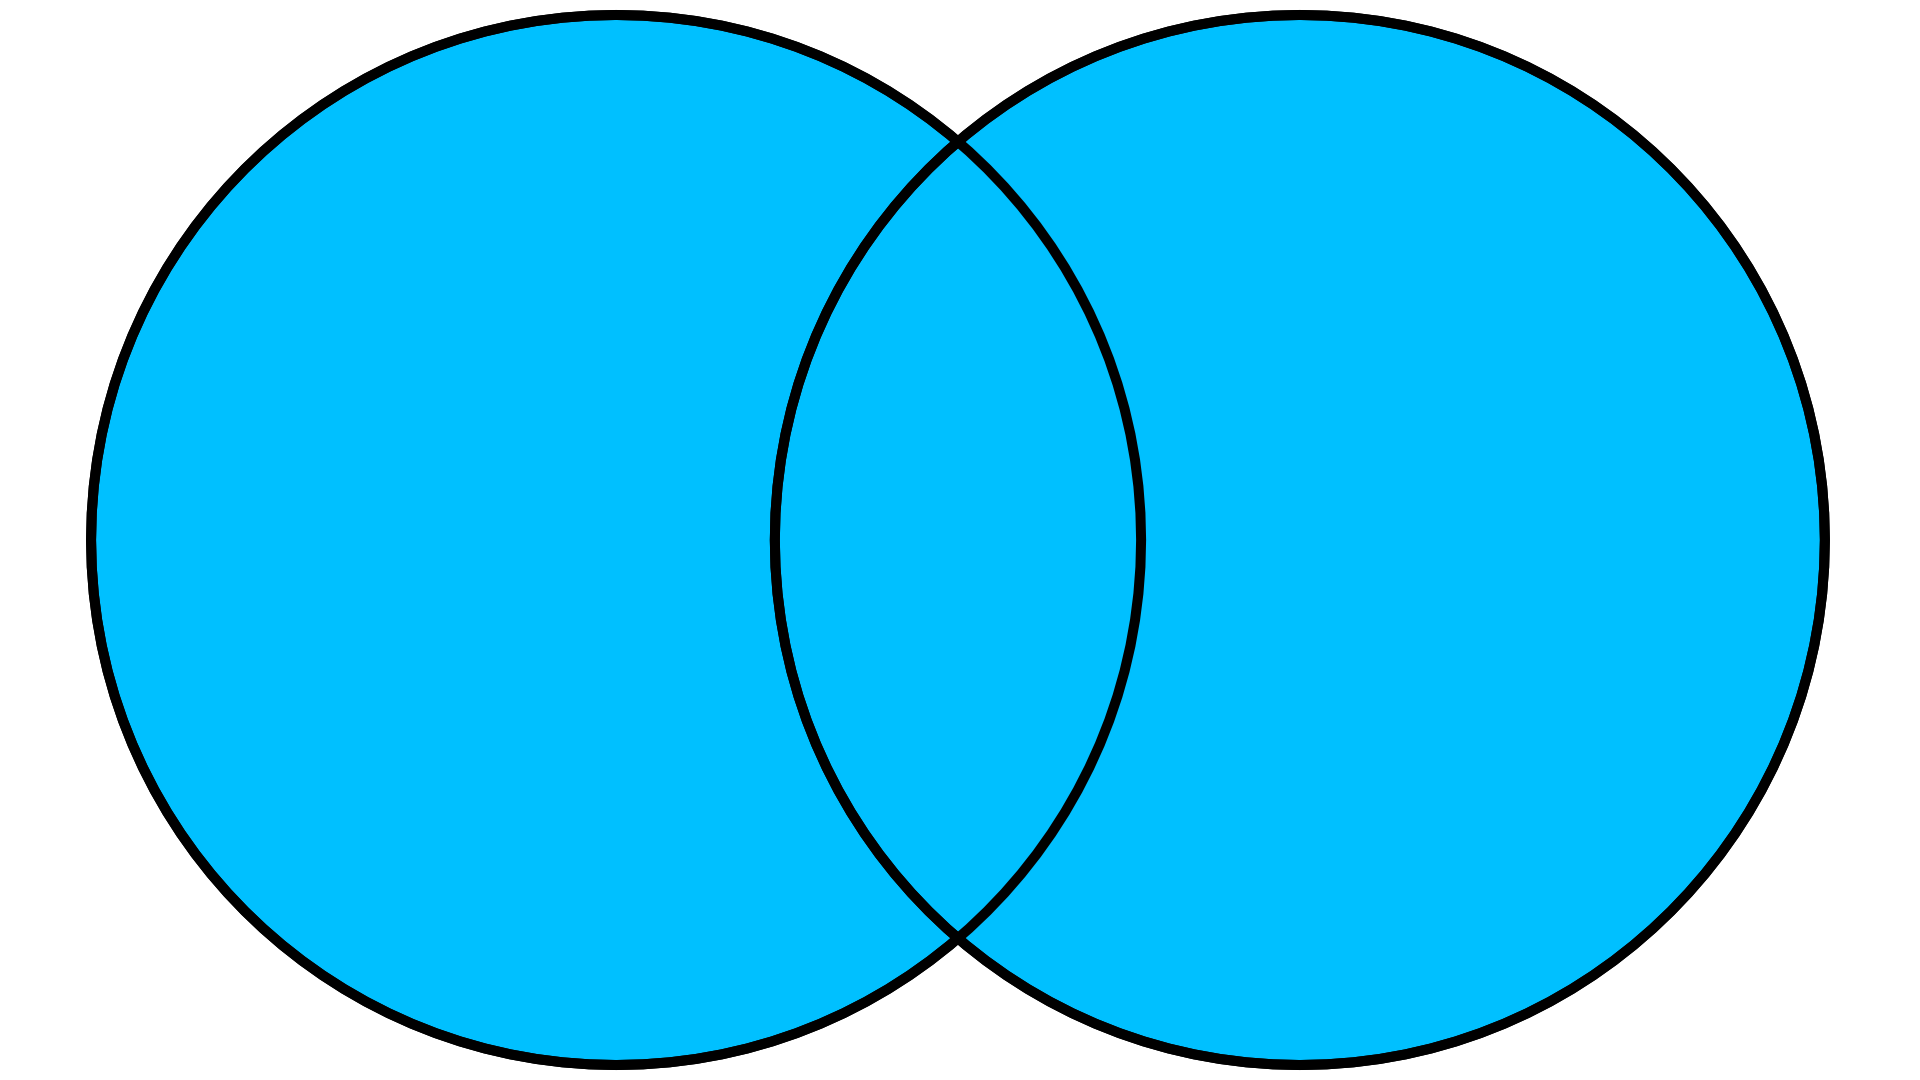
\includegraphics[width=\linewidth]{union.png}
        \end{minipage} \\
        \begin{minipage}{0.5\textwidth}
            \textbf{Differenz} $x \in A \setminus B\ \newline g.d.w.\ x \in A\ und\ x \notin B$
        \end{minipage} & 
        \begin{minipage}{0.5\textwidth}
            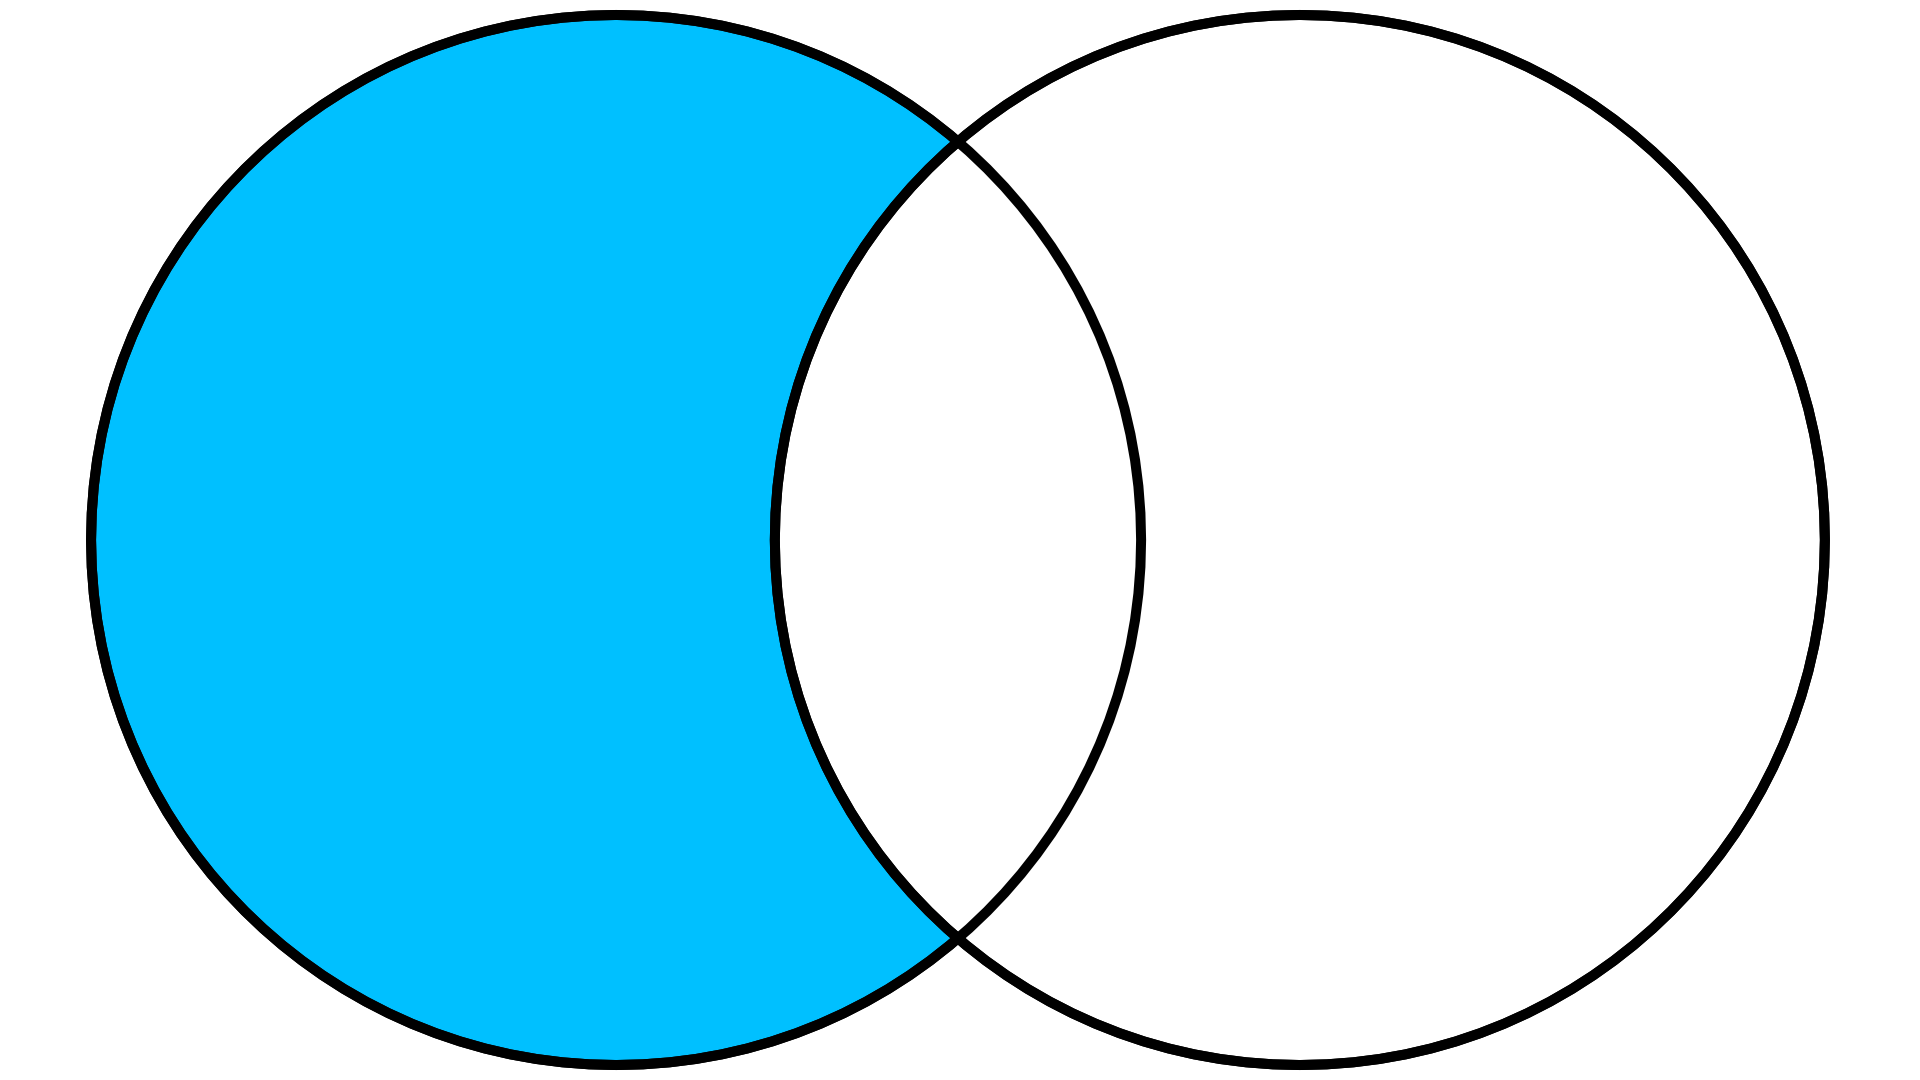
\includegraphics[width=\linewidth]{difference.png}
        \end{minipage} \\
        \begin{minipage}{0.5\textwidth}
            \textbf{Vereinigung} $x \in A \cap B\ \newline g.d.w.\ x \in A\ oder\ x \in B$
        \end{minipage} & 
        \begin{minipage}{0.5\textwidth}
            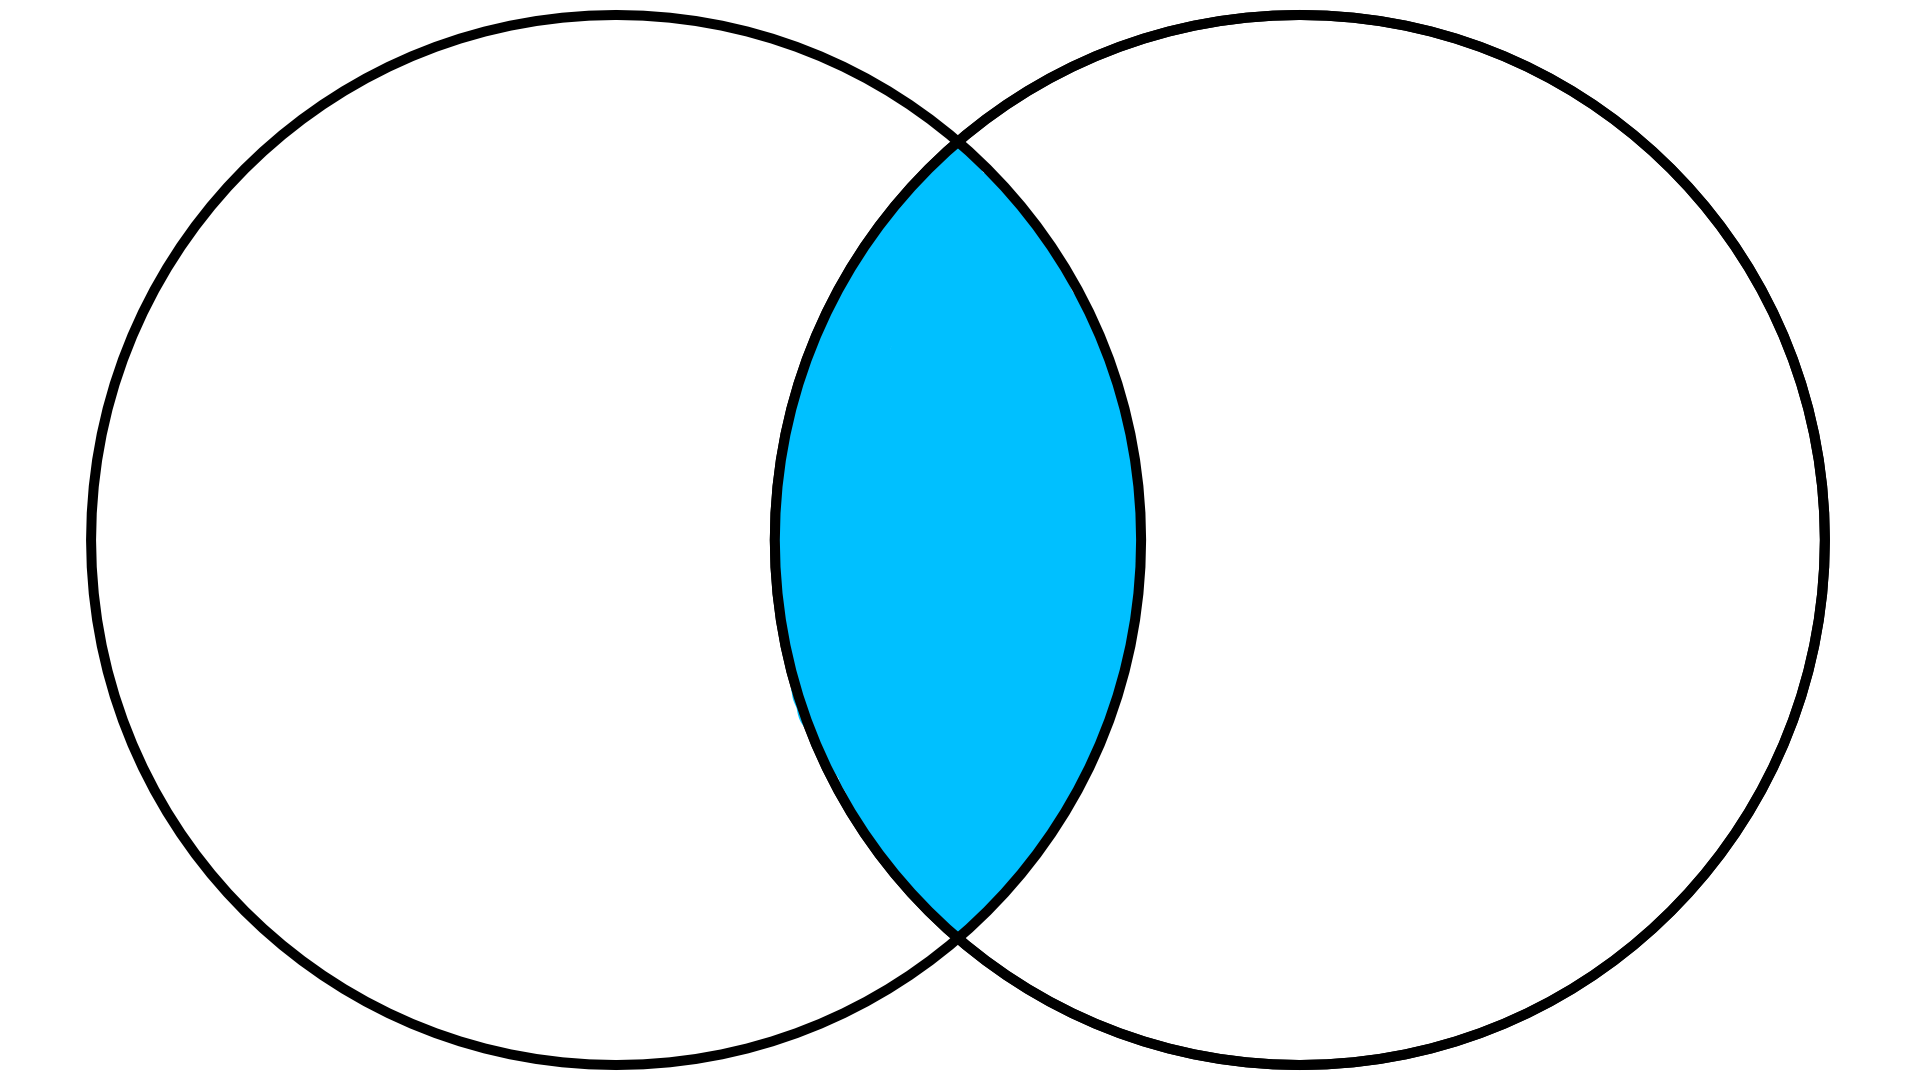
\includegraphics[width=\linewidth]{cut.png}
        \end{minipage} \\
    \end{matrix}
$
    
\end{defn}
\begin{bemerkung}
    Die Vereinigung, die Differenz und der Schnitt zweier Mengen existieren
(als neue Mengen), da sie durch das Schema der Komprehension gebildet
werden k\"onnen.
\end{bemerkung}

\begin{defn}[Relation]
    Eine Menge $R$ heisst $n$-stellige (oder $n$-\"are) Relation \"uber Mengen
    $A_1, . . . , A_n,$ falls
    \[R \subseteq \{(x_1, . . . , x_n) \mid x_1 \in A_1\ und\ \dots\ und\ x_n \in A_n\} .\]
    F\"ur eine $n$-stellige Relation $R$ \"uber Mengen $A_1, \dots , A_n$ gilt somit: Jedes
    Element von $R$ ist ein $n$-Tupel $(x_1, \dots , x_n)$ mit $x_i \in A_i$ f\"ur alle $1 \leq i \leq n$. 
\end{defn}

\begin{beispiel}
    Seien a, b und c atomare Objekte.
    \begin{itemize}
        \item $\{a, b, c\}$ ist keine Relation.
        \item $\{(a),(b),(c)\}$ ist eine Relation.
        \item $\{(a, a, a),(b, c, a),(b, c, c)\}$ ist eine Relation.
        \item $\{(a, a),(a, b, c),(c, c)\}$ ist keine Relation.

    \end{itemize}
\end{beispiel}

\begin{defn}[Kartesisches Produkt
    ]
    Eine Menge $R$ heisst $n$-stellige (oder $n$-\"are) Relation \"uber Mengen
    $A_1, . . . , A_n,$ falls
    \[R \subseteq \{(x_1, . . . , x_n) \mid x_1 \in A_1\ und\ \dots\ und\ x_n \in A_n\} .\]
    F\"ur eine $n$-stellige Relation $R$ \"uber Mengen $A_1, \dots , A_n$ gilt somit: Jedes
    Element von $R$ ist ein $n$-Tupel $(x_1, \dots , x_n)$ mit $x_i \in A_i$ f\"ur alle $1 \leq i \leq n$. 
\end{defn}
\begin{beispiel}
    Sei
    \begin{itemize}
        \item $R$ die 1-stellige Relation $R = \{(a),(b),(c)\}$ und
        \item $S$ die 2-stellige Relation $S = \{(1, 5),(2, 6)\}$.
        Dann ist $R \times S$ die 3-stellige Relation
        \[R \times S = {(a, 1, 5), (a, 2, 6), (b, 1, 5), (b, 2, 6), (c, 1, 5), (c, 2, 6)} .\]
    \end{itemize}
\end{beispiel}

\begin{bemerkung}
    Unsere Definition nennt man auch flaches kartesisches Produkt. Das
    bedeutet, dass das kartesische Produkt einer $m$-stelligen mit einer
    $n$-stelligen Relation eine ($m + n$)-stellige Relation ist.
\end{bemerkung}

\begin{bemerkung}
    Besteht $R$ aus $h$-vielen Elementen und $S$ aus $k$-vielen Elementen, so
    enth\"alt das kartesische Produkt ($h * k$)-viele Elemente.
\end{bemerkung}

\begin{bemerkung}
    \textbf{Assoziativit\"at} \newline
    Seien R, S und T Relationen. Es gilt
\[(R \times S) \times T = R \times (S \times T) .\]
Diese Eigenschaft erlaubt es uns, die Klammern wegzulassen und einfach
$R \times S \times T$ zu schreiben.

\textbf{Flaches Produkt vs. \"ubliche mathematische Definition} \newline
\"ublicherweise wird in der mathematischen Mengenlehre das kartesische
Produkt anders definiert, n\"amlich durch
\[R \times S := \{(a, b) \mid a \in R\ und\ b \in S\} . (1)\]
Damit ist $R \times S$ immer eine 2-stellige Relation. \newline
Im Gegensatz zu unserem kartesischen Produkt erf\"ullt das Produkt aus (1)
das Assoziativgesetzt nicht.
F\"ur R uns S aus dem vorherigen Beispiel finden wir dann
\[R \times S := \{((a),(1, 5)), ((a),(2, 6)), ((b),(1, 5)), ((b),(2, 6)),
((c),(1, 5)), ((c),(2, 6))\} .\]
Die Elemente aus $R \times S$ sind 2-Tupel (Paare) bestehend aus einem 1-Tupel
und einem 2-Tupel.
\end{bemerkung}
\end{document}